\documentclass[12pt,a4paper]{article}

\usepackage[utf8]{inputenc}
\usepackage[T1]{fontenc}
\usepackage[brazil]{babel}
\usepackage{geometry}
\usepackage{graphicx}
\usepackage{float}
\usepackage{booktabs}
\usepackage{array}
\usepackage{amsmath}
\usepackage{hyperref}

\geometry{margin=2.5cm}

\title{Trabalho Prático: Agente Inteligente em Labirinto}
\author{Luccas Vinicius - 20.1.8015}
\date{2026}

\begin{document}

\maketitle

\section{Introdução}

Este trabalho apresenta a implementação de um agente inteligente capaz de atuar em um labirinto discreto representado por uma matriz. O domínio foi utilizado para avaliar três abordagens de resolução de problemas em Inteligência Artificial: busca clássica, busca local e busca online.

O objetivo principal foi construir uma solução simples, funcional e explicável, permitindo comparar algoritmos, coletar métricas e analisar o comportamento do agente em diferentes condições de conhecimento do ambiente.

\section{Modelagem PEAS}

A modelagem PEAS descreve o agente em termos de desempenho, ambiente, atuadores e sensores.

\subsection{Performance}

A medida de desempenho considera que o agente deve encontrar soluções com baixo custo, menor quantidade de passos, menor número de nós expandidos e menor tempo de execução. De forma geral, o desempenho pode ser representado por:

\[
J = -\alpha \cdot custo - \beta \cdot expandidos - \gamma \cdot tempo - \delta \cdot revisitadas
\]

Quanto menor o custo, o tempo e o número de expansões, melhor é o comportamento do agente.

\subsection{Environment}

O ambiente é um labirinto em grade bidimensional. Cada célula pode representar parede, espaço livre, posição inicial, objetivo final ou ponto de coleta obrigatório. No modo online, parte do ambiente inicia desconhecida.

\subsection{Actuators}

O agente executa movimentos ortogonais:

\[
A = \{cima, baixo, esquerda, direita\}
\]

\subsection{Sensors}

Na busca clássica, o agente conhece o mapa completo. Na busca online, o agente percebe apenas uma vizinhança local e atualiza progressivamente seu mapa interno.

\section{Classificação Do Agente}

O agente implementado é baseado em objetivos e utiliza modelo interno. Ele é baseado em objetivos porque suas ações são escolhidas para alcançar o objetivo final. Ele utiliza modelo interno porque mantém uma representação do labirinto e, no modo online, atualiza essa representação conforme novas células são percebidas.

O agente também pode ser analisado como parcialmente baseado em utilidade, pois compara soluções por custo, tempo, nós expandidos e qualidade do caminho.

\section{Formulação Formal}

O problema de busca clássica foi formulado como:

\[
\langle S, A, T, s_0, G, c \rangle
\]

onde:

\begin{itemize}
    \item $S$ é o conjunto de posições livres do labirinto;
    \item $A$ é o conjunto de ações possíveis;
    \item $T$ é a função de transição entre estados;
    \item $s_0$ é a posição inicial do agente;
    \item $G$ é o teste de objetivo;
    \item $c$ é o custo de cada movimento.
\end{itemize}

Na busca local, a solução candidata é uma permutação dos pontos de coleta. O custo total da solução é a soma dos menores caminhos entre a origem, os pontos de coleta e o objetivo final.

\section{Algoritmos Implementados}

\subsection{Busca Em Largura}

A BFS explora os nós por nível. Como todos os movimentos possuem custo unitário, ela encontra o menor caminho em número de passos.

\subsection{Busca Em Profundidade}

A DFS explora um caminho até o fim antes de retroceder. Ela pode encontrar solução rapidamente, mas não garante caminho ótimo.

\subsection{Busca De Custo Uniforme}

A UCS expande primeiro o nó de menor custo acumulado. Quando todos os custos são iguais, seu comportamento tende a ser semelhante ao da BFS.

\subsection{Busca Gulosa}

A busca gulosa utiliza apenas a heurística de distância de Manhattan até o objetivo. Ela costuma ser rápida, mas não garante solução ótima.

\subsection{A Estrela}

O A* utiliza a soma do custo acumulado com a heurística:

\[
f(n) = g(n) + h(n)
\]

A heurística utilizada foi a distância de Manhattan:

\[
h(n) = |x_n - x_B| + |y_n - y_B|
\]

Essa heurística é admissível para labirintos com movimentos ortogonais e custo unitário, pois nunca superestima o custo real mínimo até o objetivo.

\section{Busca Local}

Na etapa de busca local, o agente deve visitar todos os pontos de coleta antes de alcançar o objetivo. A solução é representada pela ordem de visitação dos pontos $C$.

Foram implementados Hill-Climbing e Simulated Annealing. A vizinhança utilizada foi a troca de posição entre dois pontos de coleta. Essa escolha foi adotada por ser simples, fácil de implementar e adequada para modificar a ordem de visitação.

\subsection{Hill-Climbing}

O Hill-Climbing avalia vizinhos da solução atual e aceita apenas movimentos que reduzem o custo. Sua limitação principal é a possibilidade de ficar preso em mínimos locais.

\subsection{Simulated Annealing}

O Simulated Annealing permite aceitar soluções piores em alguns momentos, principalmente no início da execução, reduzindo a chance de ficar preso em mínimos locais. A temperatura inicial e a taxa de resfriamento influenciam diretamente a exploração.

\section{Busca Online}

Na busca online, o agente não conhece o mapa completo inicialmente. Foi implementada a estratégia de replanning com A*. O ciclo seguido pelo agente é:

\[
perceber \rightarrow atualizar \ mapa \ interno \rightarrow planejar \rightarrow agir
\]

A cada passo, o agente percebe a vizinhança local, atualiza seu mapa interno e executa A* novamente sobre o mapa parcialmente conhecido. O agente executa apenas o próximo movimento planejado e repete o processo.

\section{Metodologia Experimental}

Os algoritmos foram executados sobre um mapa textual contendo paredes, células livres, posição inicial, objetivo final e pontos de coleta. As métricas coletadas foram exportadas em arquivos CSV.

Para busca clássica, foram analisados sucesso, custo, passos, nós explorados, nós expandidos, tempo de execução e tamanho máximo da fronteira.

Para busca local, foram analisados melhor custo, pior custo, custo médio, tempo médio, número médio de iterações e taxa de sucesso.

Para busca online, foram analisados movimentos, custo real, células reveladas, células revisitadas, replanejamentos e razão entre custo online e custo ótimo offline.

\section{Resultados}

Os resultados foram gerados automaticamente na pasta \texttt{results/}. A Tabela \ref{tab:classica} apresenta o formato utilizado para comparação dos algoritmos clássicos.

\begin{table}[H]
\centering
\caption{Métricas da busca clássica}
\label{tab:classica}
\begin{tabular}{lrrrrrr}
\toprule
Algoritmo & Sucesso & Custo & Passos & Expandidos & Tempo & Fronteira \\
\midrule
BFS & Sim & - & - & - & - & - \\
DFS & Sim & - & - & - & - & - \\
UCS & Sim & - & - & - & - & - \\
Gulosa & Sim & - & - & - & - & - \\
A* & Sim & - & - & - & - & - \\
\bottomrule
\end{tabular}
\end{table}

Os valores concretos podem ser consultados nos arquivos CSV gerados pela execução do programa.

\begin{figure}[H]
\centering
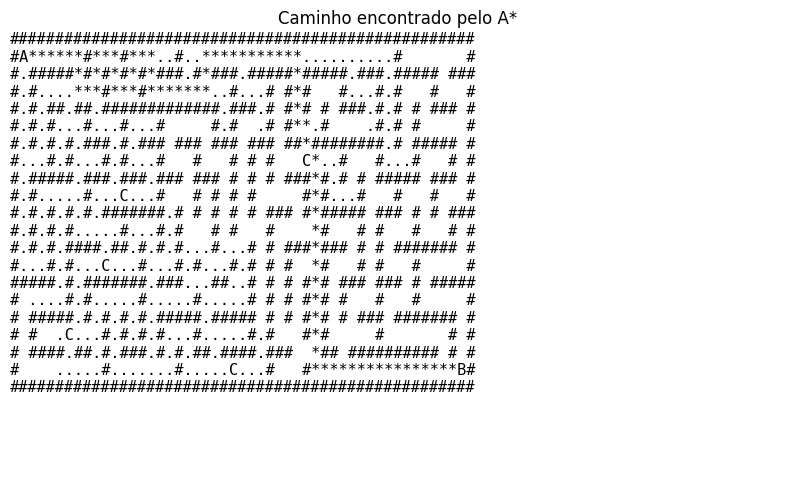
\includegraphics[width=0.90\textwidth]{../results/graficos/caminho_astar.png}
\caption{Caminho encontrado pelo algoritmo A*.}
\end{figure}

\begin{figure}[H]
\centering
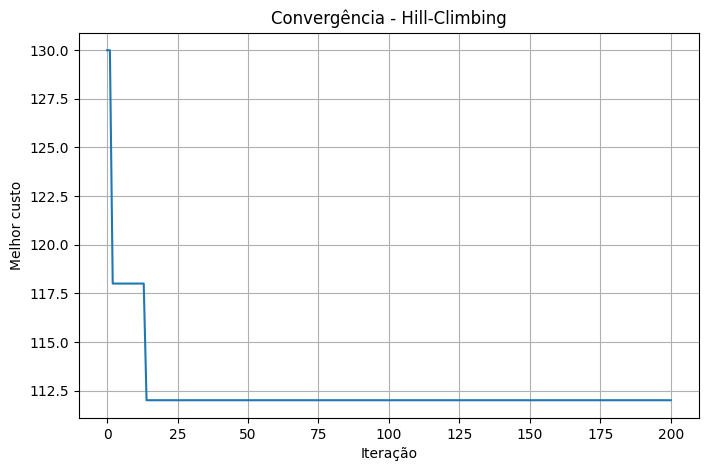
\includegraphics[width=0.90\textwidth]{../results/graficos/convergencia_hill_climbing.png}
\caption{Curva de convergência do Hill-Climbing.}
\end{figure}

\begin{figure}[H]
\centering
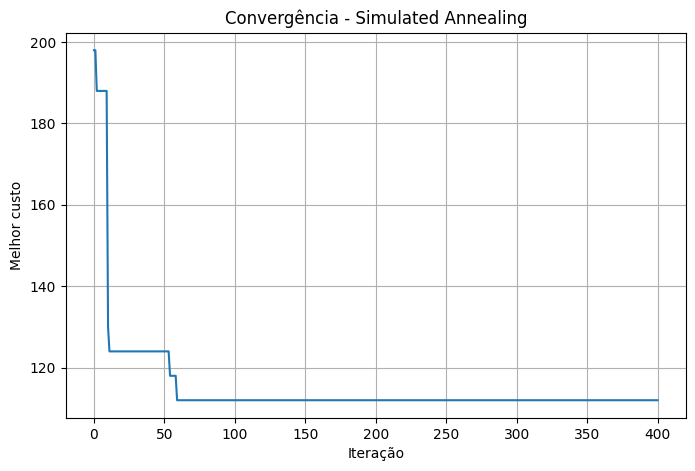
\includegraphics[width=0.90\textwidth]{../results/graficos/convergencia_simulated_annealing.png}
\caption{Curva de convergência do Simulated Annealing.}
\end{figure}

\section{Análise Crítica}

A BFS encontrou o menor caminho quando todos os movimentos tinham custo unitário, pois explora os estados por profundidade crescente. A DFS encontrou solução, mas não garante qualidade, pois pode seguir caminhos longos antes de testar alternativas melhores.

A UCS não apresentou grande diferença em relação à BFS quando todos os custos eram iguais. Caso os custos variassem, a UCS seria mais adequada, pois priorizaria o menor custo acumulado.

A busca gulosa foi eficiente, mas não é ótima, pois considera apenas a proximidade heurística do objetivo. Já o A* apresentou melhor equilíbrio entre qualidade da solução e eficiência, pois combina custo acumulado e heurística.

Na busca local, o Hill-Climbing pode ficar preso em mínimo local, pois aceita apenas melhorias. O Simulated Annealing tende a ser mais robusto porque aceita soluções piores de forma controlada, principalmente no início da execução.

Na busca online, o agente pode tomar decisões subótimas porque não conhece o mapa completo. A razão online/offline mede o custo pago pela falta de conhecimento inicial do ambiente.

\section{Limitações}

A solução utiliza mapas pequenos e custo unitário de movimento. A visualização é simples, baseada em imagens estáticas. A busca online utiliza uma estratégia básica de replanning e pode ser melhorada com técnicas mais sofisticadas de exploração de fronteiras.

\section{Uso De IA}

Foi utilizada IA generativa como ferramenta de apoio para estruturar o código, revisar conceitos e auxiliar na documentação. O uso foi registrado no arquivo \texttt{uso\_ia.md}. A solução foi validada por execução prática e geração de métricas.

\section{Conclusão}

O trabalho permitiu comparar diferentes estratégias de busca em um mesmo domínio. A busca clássica foi adequada quando o mapa era conhecido. A busca local foi utilizada para otimizar a ordem dos pontos de coleta. A busca online demonstrou o impacto da falta de conhecimento inicial do ambiente, exigindo percepção, atualização do modelo interno e replanejamento contínuo.

\end{document}
